
%% bare_conf.tex
%% V1.3
%% 2007/01/11
%% by Michael Shell
%% See:
%% http://www.michaelshell.org/
%% for current contact information.
%%
%% This is a skeleton file demonstrating the use of IEEEtran.cls
%% (requires IEEEtran.cls version 1.7 or later) with an IEEE conference paper.
%%
%% Support sites:
%% http://www.michaelshell.org/tex/ieeetran/
%% http://www.ctan.org/tex-archive/macros/latex/contrib/IEEEtran/
%% and
%% http://www.ieee.org/

%%*************************************************************************
%% Legal Notice:
%% This code is offered as-is without any warranty either expressed or
%% implied; without even the implied warranty of MERCHANTABILITY or
%% FITNESS FOR A PARTICULAR PURPOSE! 
%% User assumes all risk.
%% In no event shall IEEE or any contributor to this code be liable for
%% any damages or losses, including, but not limited to, incidental,
%% consequential, or any other damages, resulting from the use or misuse
%% of any information contained here.
%%
%% All comments are the opinions of their respective authors and are not
%% necessarily endorsed by the IEEE.
%%
%% This work is distributed under the LaTeX Project Public License (LPPL)
%% ( http://www.latex-project.org/ ) version 1.3, and may be freely used,
%% distributed and modified. A copy of the LPPL, version 1.3, is included
%% in the base LaTeX documentation of all distributions of LaTeX released
%% 2003/12/01 or later.
%% Retain all contribution notices and credits.
%% ** Modified files should be clearly indicated as such, including  **
%% ** renaming them and changing author support contact information. **
%%
%% File list of work: IEEEtran.cls, IEEEtran_HOWTO.pdf, bare_adv.tex,
%%                    bare_conf.tex, bare_jrnl.tex, bare_jrnl_compsoc.tex
%%*************************************************************************

% *** Authors should verify (and, if needed, correct) their LaTeX system  ***
% *** with the testflow diagnostic prior to trusting their LaTeX platform ***
% *** with production work. IEEE's font choices can trigger bugs that do  ***
% *** not appear when using other class files.                            ***
% The testflow support page is at:
% http://www.michaelshell.org/tex/testflow/



% Note that the a4paper option is mainly intended so that authors in
% countries using A4 can easily print to A4 and see how their papers will
% look in print - the typesetting of the document will not typically be
% affected with changes in paper size (but the bottom and side margins will).
% Use the testflow package mentioned above to verify correct handling of
% both paper sizes by the user's LaTeX system.
%
% Also note that the "draftcls" or "draftclsnofoot", not "draft", option
% should be used if it is desired that the figures are to be displayed in
% draft mode.
%
\documentclass[10pt, conference, compsocconf]{IEEEtran}
% Add the compsocconf option for Computer Society conferences.
%
% If IEEEtran.cls has not been installed into the LaTeX system files,
% manually specify the path to it like:
% \documentclass[conference]{../sty/IEEEtran}





% Some very useful LaTeX packages include:
% (uncomment the ones you want to load)


% *** MISC UTILITY PACKAGES ***
%
%\usepackage{ifpdf}
% Heiko Oberdiek's ifpdf.sty is very useful if you need conditional
% compilation based on whether the output is pdf or dvi.
% usage:
% \ifpdf
%   % pdf code
% \else
%   % dvi code
% \fi
% The latest version of ifpdf.sty can be obtained from:
% http://www.ctan.org/tex-archive/macros/latex/contrib/oberdiek/
% Also, note that IEEEtran.cls V1.7 and later provides a builtin
% \ifCLASSINFOpdf conditional that works the same way.
% When switching from latex to pdflatex and vice-versa, the compiler may
% have to be run twice to clear warning/error messages.






% *** CITATION PACKAGES ***
%
\usepackage{cite}
% cite.sty was written by Donald Arseneau
% V1.6 and later of IEEEtran pre-defines the format of the cite.sty package
% \cite{} output to follow that of IEEE. Loading the cite package will
% result in citation numbers being automatically sorted and properly
% "compressed/ranged". e.g., [1], [9], [2], [7], [5], [6] without using
% cite.sty will become [1], [2], [5]--[7], [9] using cite.sty. cite.sty's
% \cite will automatically add leading space, if needed. Use cite.sty's
% noadjust option (cite.sty V3.8 and later) if you want to turn this off.
% cite.sty is already installed on most LaTeX systems. Be sure and use
% version 4.0 (2003-05-27) and later if using hyperref.sty. cite.sty does
% not currently provide for hyperlinked citations.
% The latest version can be obtained at:
% http://www.ctan.org/tex-archive/macros/latex/contrib/cite/
% The documentation is contained in the cite.sty file itself.






% *** GRAPHICS RELATED PACKAGES ***
%
\ifCLASSINFOpdf
   \usepackage[pdftex]{graphicx}
  % declare the path(s) where your graphic files are
   \graphicspath{{../pdf/}{../jpeg/}}
  % and their extensions so you won't have to specify these with
  % every instance of \includegraphics
   \DeclareGraphicsExtensions{.pdf,.jpeg,.png}
\else
  % or other class option (dvipsone, dvipdf, if not using dvips). graphicx
  % will default to the driver specified in the system graphics.cfg if no
  % driver is specified.
   \usepackage[dvips]{graphicx}
  % declare the path(s) where your graphic files are
   \graphicspath{{./}}
  % and their extensions so you won't have to specify these with
  % every instance of \includegraphics
   \DeclareGraphicsExtensions{.png, .pdf, .eps}
\fi
% graphicx was written by David Carlisle and Sebastian Rahtz. It is
% required if you want graphics, photos, etc. graphicx.sty is already
% installed on most LaTeX systems. The latest version and documentation can
% be obtained at: 
% http://www.ctan.org/tex-archive/macros/latex/required/graphics/
% Another good source of documentation is "Using Imported Graphics in
% LaTeX2e" by Keith Reckdahl which can be found as epslatex.ps or
% epslatex.pdf at: http://www.ctan.org/tex-archive/info/
%
% latex, and pdflatex in dvi mode, support graphics in encapsulated
% postscript (.eps) format. pdflatex in pdf mode supports graphics
% in .pdf, .jpeg, .png and .mps (metapost) formats. Users should ensure
% that all non-photo figures use a vector format (.eps, .pdf, .mps) and
% not a bitmapped formats (.jpeg, .png). IEEE frowns on bitmapped formats
% which can result in "jaggedy"/blurry rendering of lines and letters as
% well as large increases in file sizes.
%
% You can find documentation about the pdfTeX application at:
% http://www.tug.org/applications/pdftex





% *** MATH PACKAGES ***
%
%\usepackage[cmex10]{amsmath}
% A popular package from the American Mathematical Society that provides
% many useful and powerful commands for dealing with mathematics. If using
% it, be sure to load this package with the cmex10 option to ensure that
% only type 1 fonts will utilized at all point sizes. Without this option,
% it is possible that some math symbols, particularly those within
% footnotes, will be rendered in bitmap form which will result in a
% document that can not be IEEE Xplore compliant!
%
% Also, note that the amsmath package sets \interdisplaylinepenalty to 10000
% thus preventing page breaks from occurring within multiline equations. Use:
%\interdisplaylinepenalty=2500
% after loading amsmath to restore such page breaks as IEEEtran.cls normally
% does. amsmath.sty is already installed on most LaTeX systems. The latest
% version and documentation can be obtained at:
% http://www.ctan.org/tex-archive/macros/latex/required/amslatex/math/





% *** SPECIALIZED LIST PACKAGES ***
%
%\usepackage{algorithmic}
% algorithmic.sty was written by Peter Williams and Rogerio Brito.
% This package provides an algorithmic environment fo describing algorithms.
% You can use the algorithmic environment in-text or within a figure
% environment to provide for a floating algorithm. Do NOT use the algorithm
% floating environment provided by algorithm.sty (by the same authors) or
% algorithm2e.sty (by Christophe Fiorio) as IEEE does not use dedicated
% algorithm float types and packages that provide these will not provide
% correct IEEE style captions. The latest version and documentation of
% algorithmic.sty can be obtained at:
% http://www.ctan.org/tex-archive/macros/latex/contrib/algorithms/
% There is also a support site at:
% http://algorithms.berlios.de/index.html
% Also of interest may be the (relatively newer and more customizable)
% algorithmicx.sty package by Szasz Janos:
% http://www.ctan.org/tex-archive/macros/latex/contrib/algorithmicx/




% *** ALIGNMENT PACKAGES ***
%
%\usepackage{array}
% Frank Mittelbach's and David Carlisle's array.sty patches and improves
% the standard LaTeX2e array and tabular environments to provide better
% appearance and additional user controls. As the default LaTeX2e table
% generation code is lacking to the point of almost being broken with
% respect to the quality of the end results, all users are strongly
% advised to use an enhanced (at the very least that provided by array.sty)
% set of table tools. array.sty is already installed on most systems. The
% latest version and documentation can be obtained at:
% http://www.ctan.org/tex-archive/macros/latex/required/tools/


%\usepackage{mdwmath}
%\usepackage{mdwtab}
% Also highly recommended is Mark Wooding's extremely powerful MDW tools,
% especially mdwmath.sty and mdwtab.sty which are used to format equations
% and tables, respectively. The MDWtools set is already installed on most
% LaTeX systems. The lastest version and documentation is available at:
% http://www.ctan.org/tex-archive/macros/latex/contrib/mdwtools/


% IEEEtran contains the IEEEeqnarray family of commands that can be used to
% generate multiline equations as well as matrices, tables, etc., of high
% quality.


%\usepackage{eqparbox}
% Also of notable interest is Scott Pakin's eqparbox package for creating
% (automatically sized) equal width boxes - aka "natural width parboxes".
% Available at:
% http://www.ctan.org/tex-archive/macros/latex/contrib/eqparbox/





% *** SUBFIGURE PACKAGES ***
%\usepackage[tight,footnotesize]{subfigure}
% subfigure.sty was written by Steven Douglas Cochran. This package makes it
% easy to put subfigures in your figures. e.g., "Figure 1a and 1b". For IEEE
% work, it is a good idea to load it with the tight package option to reduce
% the amount of white space around the subfigures. subfigure.sty is already
% installed on most LaTeX systems. The latest version and documentation can
% be obtained at:
% http://www.ctan.org/tex-archive/obsolete/macros/latex/contrib/subfigure/
% subfigure.sty has been superceeded by subfig.sty.



%\usepackage[caption=false]{caption}
%\usepackage[font=footnotesize]{subfig}
% subfig.sty, also written by Steven Douglas Cochran, is the modern
% replacement for subfigure.sty. However, subfig.sty requires and
% automatically loads Axel Sommerfeldt's caption.sty which will override
% IEEEtran.cls handling of captions and this will result in nonIEEE style
% figure/table captions. To prevent this problem, be sure and preload
% caption.sty with its "caption=false" package option. This is will preserve
% IEEEtran.cls handing of captions. Version 1.3 (2005/06/28) and later 
% (recommended due to many improvements over 1.2) of subfig.sty supports
% the caption=false option directly:
%\usepackage[caption=false,font=footnotesize]{subfig}
%
% The latest version and documentation can be obtained at:
% http://www.ctan.org/tex-archive/macros/latex/contrib/subfig/
% The latest version and documentation of caption.sty can be obtained at:
% http://www.ctan.org/tex-archive/macros/latex/contrib/caption/




% *** FLOAT PACKAGES ***
%
%\usepackage{fixltx2e}
% fixltx2e, the successor to the earlier fix2col.sty, was written by
% Frank Mittelbach and David Carlisle. This package corrects a few problems
% in the LaTeX2e kernel, the most notable of which is that in current
% LaTeX2e releases, the ordering of single and double column floats is not
% guaranteed to be preserved. Thus, an unpatched LaTeX2e can allow a
% single column figure to be placed prior to an earlier double column
% figure. The latest version and documentation can be found at:
% http://www.ctan.org/tex-archive/macros/latex/base/



%\usepackage{stfloats}
% stfloats.sty was written by Sigitas Tolusis. This package gives LaTeX2e
% the ability to do double column floats at the bottom of the page as well
% as the top. (e.g., "\begin{figure*}[!b]" is not normally possible in
% LaTeX2e). It also provides a command:
%\fnbelowfloat
% to enable the placement of footnotes below bottom floats (the standard
% LaTeX2e kernel puts them above bottom floats). This is an invasive package
% which rewrites many portions of the LaTeX2e float routines. It may not work
% with other packages that modify the LaTeX2e float routines. The latest
% version and documentation can be obtained at:
% http://www.ctan.org/tex-archive/macros/latex/contrib/sttools/
% Documentation is contained in the stfloats.sty comments as well as in the
% presfull.pdf file. Do not use the stfloats baselinefloat ability as IEEE
% does not allow \baselineskip to stretch. Authors submitting work to the
% IEEE should note that IEEE rarely uses double column equations and
% that authors should try to avoid such use. Do not be tempted to use the
% cuted.sty or midfloat.sty packages (also by Sigitas Tolusis) as IEEE does
% not format its papers in such ways.





% *** PDF, URL AND HYPERLINK PACKAGES ***
%
%\usepackage{url}
% url.sty was written by Donald Arseneau. It provides better support for
% handling and breaking URLs. url.sty is already installed on most LaTeX
% systems. The latest version can be obtained at:
% http://www.ctan.org/tex-archive/macros/latex/contrib/misc/
% Read the url.sty source comments for usage information. Basically,
% \url{my_url_here}.





% *** Do not adjust lengths that control margins, column widths, etc. ***
% *** Do not use packages that alter fonts (such as pslatex).         ***
% There should be no need to do such things with IEEEtran.cls V1.6 and later.
% (Unless specifically asked to do so by the journal or conference you plan
% to submit to, of course. )


% correct bad hyphenation here
\hyphenation{op-tical net-works semi-conduc-tor}


\begin{document}
%
% paper title
% can use linebreaks \\ within to get better formatting as desired
\title{Libvina: A Template Approach to Specialize sources for Multicore Architectures}


% author names and affiliations
% use a multiple column layout for up to two different
% affiliations

%\author{\IEEEauthorblockN{Authors Name/s per 1st Affiliation (Author)}
%\IEEEauthorblockA{line 1 (of Affiliation): dept. name of organization\\
%line 2: name of organization, acronyms acceptable\\
%line 3: City, Country\\
%line 4: Email: name@xyz.com}
%\and
%\IEEEauthorblockN{Authors Name/s per 2nd Affiliation (Author)}
%\IEEEauthorblockA{line 1 (of Affiliation): dept. name of organization\\
%line 2: name of organization, acronyms acceptable\\
%line 3: City, Country\\
%line 4: Email: name@xyz.com}
%}

% conference papers do not typically use \thanks and this command
% is locked out in conference mode. If really needed, such as for
% the acknowledgment of grants, issue a \IEEEoverridecommandlockouts
% after \documentclass

% for over three affiliations, or if they all won't fit within the width
% of the page, use this alternative format:
% 
\author{\IEEEauthorblockN{Xin Liu}}




% use for special paper notices
%\IEEEspecialpapernotice{(Invited Paper)}




% make the title area
\maketitle


\begin{abstract}
We introduce libvina -- a template library designed to specialize programs for different architectures. A source-to-source compilation is helpful to change programs more closer to contemporary multicore hardwares. We proposed a new approach to achieve this target for problems with rich static information. In libvina, parallelization and optimization of memory hierarchy are conducted by a groups of C++ template classes. It is flexible and extensible. Programmers with decent knowledge of template meta-programming are capable to extend library. Because template library effects in compiler time, minimal runtime cost is incurred from our approach. Finally, We evaluate the effects of specialization of some typical applications in multimedia and scientific computation on commodity x86 and GPU platforms.
\end{abstract}

\begin{IEEEkeywords}
static analysis; Compiler optimization; parallelization
\end{IEEEkeywords}


% For peer review papers, you can put extra information on the cover
% page as needed:
% \ifCLASSOPTIONpeerreview
% \begin{center} \bfseries EDICS Category: 3-BBND \end{center}
% \fi
%
% For peerreview papers, this IEEEtran command inserts a page break and
% creates the second title. It will be ignored for other modes.
\IEEEpeerreviewmaketitle

\section{Introduction}
In multicore period, hardware architects rely on parallelism and memory hierarchy to enhance performance. Both cloned processors and elaborated storage-on-chip require programmer to restructure their source code and keep tuning binaries for a specific target.Therefore, writing a high-performance application requires non-trivial knowledge of underlying machine's architecture. The gap between hardware vendors and software developers extends development cycle, which increases marketing cost and risks for innovative multicore architectures in silicon industry.

Algorithm experts usually focus on their specific domains and have limited insights on diverging computer systems. They expect hardware and optimized compiler to guarantee decent performance for their programs. The expectation was roughly held until massive parallelization was introduced to computer community. Since frequency of general purpose processor stops growing faster, it's hard for legacy software to obtain performance enhancement from hardware's refinement freely. Plain C/C++ can not fully reflect contemplate architecture any more. Researchers have admitted that it is tremendously challenging for optimizing sequential code by a compiler, so the answer to bridge programmer to parallel hardware relies on language and library to express concurrency richer than ever.

Designing new parallel programming is possible. Many functional languages \cite{13} with inherent concurrency supports have emerged to the horizon of computer. However, a conservative programmer may turn them down because there are still lack of convincing evidences to demonstrate programmability and efficiency comparing to traditional programming languages. Another reason is software cost. Considering the time span which a large computer system serves, hardwares are cheap and become cheaper with time passing; software and personnel with well-trained programming knowledge are expensive. Even numerous legacy systems designed without consideration of multi-threaded environment at that time, vendors usually prefer to update and maintain software systems for current and future hardwares rather than restarting from scratch. 

One side, software developers insist on classic programming diagrams and are reluctant to rewrite all the existing sources. On the other side, utilizing the powerhouse of modern processors to boost performance for existing and new systems is an important issue for them. Therefore, it is desirable to extend traditional programming languages to honor the trade-off.

Many programming languages extending popular programming languages had been proposed for multicore. However, most of existing solutions aimed at specific architectures or computer systems. \textit{e.g.} CUDA only works on vender-dependent GPU architecture; UPC and OpenMP are designed for shared memory system \cite{15}. Sequoia \cite{1} is an attempt to customize code-generation rule by XML configuration, however, it follows the similar restriction because it enforces programmer to model target as a tree of abstract machines.

Our approach is similar to Sequoia and OpenMP to perform source-to-source transformation by compiler. We shared the same idea of cite{1} to generate a cluster of subprocedures for a task recursively. Instead of modifying compiler and introducing new language constructs, we exploit the capability of C++ template mechanism to achieve translation. All transformation rules are programmed in C++ meta-programming \cite{10}.  In libvina, a primary limitation is that only type and static constant value are available in compiler time. Therefore, it only works for problems which have rich static information. Fortunately, applications with this attributions are numerous in multimedia, digital processing, and scientific computations 

Because libvina effects in compiler time, it is possible to avoid from deploying runtime system, which means that it can incur minimal runtime cost if applications allow. Another advantage of template approach is that it imposes less restricts comparing with other static approaches:

\begin{itemize}
\item Thread-independent:  It is possible to generate all kind of threads for target, including pthread, native LWP provided by OS, even vendor-dependent thread. 

\item Execution-independent:  Our approach does not bind to any execution model. Libvina can change program to SPMD threads to exploit parallelism from multicore; link many subroutines to build a pipeline to hide latency of memory; or separate our program into blocks to improve locality. 

\item Extendability:  It is flexible to develop new template class to utilize new architectural features. Template meta-programming is intimate for C++ experts. It's easy to extend new execution rules and parallel patterns. Another approaches have to ratify languages and then modify compiler to add features.

\item Portability: Template mechanism are standardized in ISO \cite{8, 17}. Our template library conforms to standards and is guaranteed to be portable for all mainstreaming C++ compilers.
\end{itemize}

The remaining parts of this paper are structured as follows. Section 2 summarizes some related works on static transformation and other library-based solutions. Section 3 introduces fundamentals of libvina. Then Section 4 represents some typical transformations in libvina. Experiments and results are in Section 5 to evaluate effect of transformations. Final section is conclusion and future works.

\section{Related work}
As mentioned before, it is desirable to extend conventional programming languages to reflects the essence of newer hardware. Researches in the field have two major directions:
\begin{enumerate}
\item providing new library to support programming in concurrency
\item extending language constructs to extend parallel semantics
\end{enumerate}

First, library is a common method to extend language capability without introducing new language constructs or modifying grammar. POSIX thread library is a de facto standard interface to utilize multi-thread for applications on UNIX-like systems. The relationship between pthread and native thread provided by OS is straightforward. Therefore, abstraction of pthread is far away from naturally expressing parallelism and concurrency. Furthermore, the implementation of thread on hardware is unspecific in the standard, so it can not guarantee performance or even correctness on some architectures \cite{4, 5}

C++ community intends to develop parallel library while bearing generic programming in mind. TBB(Thread Block Builder) has a plenty of containers and execution rules. Entities including partitioner and scheduler in TBB are created in runtime. In that case, key data structures have to be thread-safe. Although TBB exploits task parallelism or other sophisticated concurrency on general purpose processors, the runtime overhead is relative high in data parallel programs, especially in the scenario that massive ALUs are exposed by hardware. Solution we proposed here is orthogonal to runtime parallel libraries. We only exploit parallelism that can be determined in static time, developers feel free to resort to other ways to speedup the programs in runtime, such as TBB.
 
%% MPI
%Another dominant parallel library is MPI in supercomputing community. It based on message-passing mechanism and SPMD model to execute parallel program. The difficulties of developing MPI programs are as notorious as pthread counterpart for programmers without sufficent training of parallel programming. 
%%

Second, language communities extend their semantics by modifying compiler. They could add directive or annotation to help compiler transform source code. OpenMP is designed for shared memory and has shipped in almost every C/Fortran compilers. OMP compilers transform sequential code into multi-threaded programs with OMP runtime. Although OpenMP is simple and portable, the performance is not optimal in most cases. A handful of directives leave small room for further enhancing program and scaling up to larger systems. Hybrid OpenMP with MPI is possible, but difficulty surges.

Another approach needing to modify compiler is to add new language constructs. Sequoia is a source-to-source compiler to support programming memory hierarchy. First of all, It targets execution environment as a tree of machines, which an individual machine owns its storage and computation unit. Second, It terms a computation-intensive function as \textit{task}. New constructs apply on \emph{task}. Sequoia compiler transforms a \textit{task} into a cluster of subprocedures based on machines hierarchy. The target machines are described in XML files. Based on this idea, Sequoia actually can specialize task for target architectures. \cite{2} reports Sequoia can successfully transform codes for CellBE, SMP, cluster while keeping very competitive performance. However, Sequoia as a language extension is restrictive. The basic data structure is array, which obviously shows the preference of scientific computation. The language constructs do not cover all the common parallel patterns such as pipeline and task queue. Libvina derived the idea of Sequoia to transform source code recursively. However, template meta-programming utilizes existing mechanism in C++ compiler and is capable to express all the semantics in Sequoia programming language. Moreover, Sequoia can not leverage type system to specialize code. \textit{e.g.} Many modern processors usually provide SIMD instructions. Libvina could generate corresponding source based on predefined vector types. Sequoia compiler ignores this important information and simply relies on following compiler.

With the astonishing pace of core proliferation and architecture refinement, GPU has evolved to a pioneer of supercomputing. OpenCL \cite{12} programming language is strongly affected by vender-dependent predecessor CUDA. It provides a unified computation platform. The downside of OpenCL is the obvious bias toward Streaming architectures. Because OpenCL has to assume its simplest computation unit for target, recursion in kernel function is forbidden in the specification. It is regarded as a simple and neat way to divide problems. Libvina can cooperate with OpenCL to transform code for GPU. It recursively generates tasks and finally emit OpenCL kernel programs while hiding details to user programming. 

\section{Mechanism of libvina}
\subsection{template meta-programming approach}
Originally, C++ template mechanism is invented to supersede C preprocessor. It is type-safe and could facility generic programming. People found the potential of template computation by chance. \cite{6} later proved template itself is Turing completeness. 

Template meta-programming is similar to functional programming language except it effects in compiler time. It only relies on static information to determine control flow and perform computation. Beside the job it meant to do, template has successfully applied to many innovative purposes in modern C++ programming practices \cite{9}. MPL Library \cite{16} provides control statement and STL-like data structures, which greatly eases programming in static realm.

\subsection{Concepts}
In libvina, we assume C++ compiler front-end with template mechanism as a code generator. It actually practices source-to-source transformation in the guidance of meta-programming. 

%TF class
Libvina focuses on computation-intensive functions which are commonly referred to \emph{kernel} or \emph{filter}. Mathematically, a function is single-target binary relation. Kernel functions are usually self-contained, \textit{i.e.} external data references are limited and calling graphs are simple. It's possible for a kernel function to decouple into a group of subprocedures. Each subprocedure may be exactly the same as kernel and spread on multicore running in parallel.  Another approach is to divide a kernel into finer stages and run in streaming manner to respect data locality and bandwidth. In libvina, a \emph{transform class (TF class)} is a template class which transforms a function to a cluster of subprocedures in isomorphism. As shown in ~\ref{fig:tfcls}, the transformed function on right side has the same interface while owns a call graph to complete the original computation by a cluster of subprocedures. Execution of the call graph can be programmed by in the library to scrutinise target's architecture.

\begin{figure}
\centering
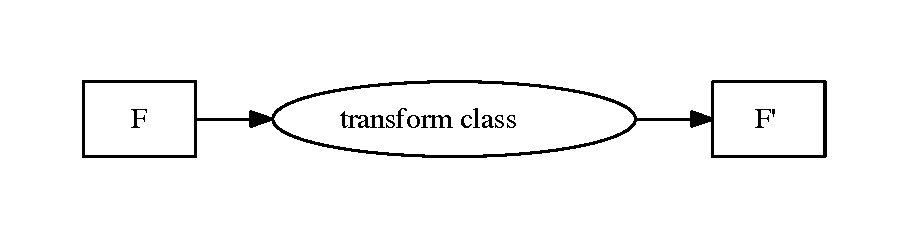
\includegraphics[width=3.3in]{map-class}
\caption{transform class}
\label{fig:tfcls}
\end{figure}

%predicate and sentinel
Borrowed from lisp concept, \emph{predicate} represents a indicator of some conditions. In libvina, it is a template class with static fields initialized by constant expressions consisting of template parameters and constants. These fields are automatically evaluated when template classes are instantiated. ~\ref{lst:pred} is an example to determine whether the problem size is fitting to last level cache.

\makebox[3.1\width]{\hrulefill}
\begin{verbatim}
template <class T, int SIZE_A
     , int SIZE_B, int SIZE_C>
struct p_lt_cache_ll {
 enum {CACHE_LL_SIZE = 4096*1024};
 const static bool value = 
     ((SIZE_A * SIZE_B 
   + SIZE_A * SIZE_C + SIZE_B * SIZE_C) 
   * sizeof(T) ) <= CACHE_LL_SIZE;
};
\end{verbatim}
\begin{center}
\caption{List - 1 : predicate lt\_cache\_ll}
\label{lst:pred}
\end{center}

\emph{Sentinels} in libvina are non-type template parameters of \emph{TF class}, with a \emph{predicate} as default initializer. When a template class is instantiating, sentinels are evaluated.  A \emph{predicate} determines whether a specific requirement has been satisfied. Sentinel is responsible for changing generation strategy according to the result. C++ compiler chooses different versions of a template class to instantiates basing on the values or types of template arguments. This mechanism is known as \emph{specialization}.

%view
Template meta-programing can only manipulate static information. As a result, ADTs in libvina need to carry information such as dimensionality as template parameters. Only Vector and Matrix are implemented in our library, because they cover a wide spectrum of application in multimedia area. Users require more versatile data structures could resort to \cite{10}. As ~\ref{fig:view} depicted, View is a concept to abstract dataset in libvina. It is divisible and type-safe. Shadow region is the other thread space. The only approach to communicate with other thread is through ViewMT. It guarantees synchronization by signal mechanism internally. We only provide synchronizations for data set to encourage block operations.  

\begin{figure}
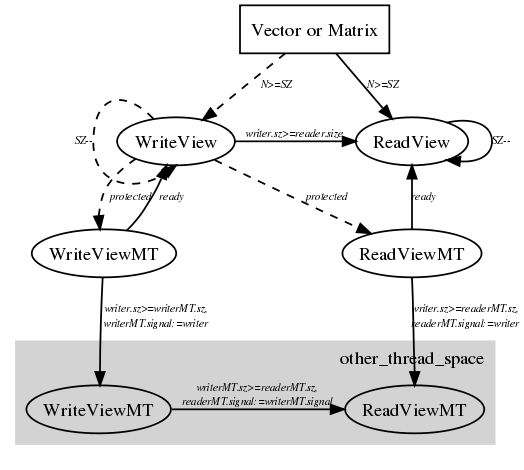
\includegraphics[width=3.3in]{view_concept}
\caption{View}
\label{fig:view}
\end{figure}

%
\section{Program specialization}
\subsection{Multi-threaded}
Multi-threading is dominant approach to utilize duplicated computation units.  There are numerous kernel functions in multimedia applications and scientific computations which can easily exploit data parallelism by dividing task into smaller and independent subtasks. This feature naturally matches libvina's transformation. We implemented \emph{mappar} and \emph{mapreduce} language constructs in \cite{1} as template classes. 

~\ref{lst:mappar} is the definition of \emph{mappar} TF class. Template parameter \emph{Instance} is computation task containing kernel function wrapper and arguments. The last template parameter \emph{\_\_SENTINEL\_\_} determines control flow when internalization occurs. ~\ref{lst-mappar2} is a specialization to generate concrete thread to practice computation. It is noteworthy that the last two arguments are \emph{true}, which means that this class is multi-threaded and leaf node version. 

\makebox[3.1\width]{\hrulefill}
\begin{verbatim}
template <class Instance, int  _K,
	  bool _IsMT,  bool __SENTINEL__>
struct mappar {
typedef mappar<typename Instance::SubTask, 
        _K, _IsMT, 
	Instance::SubTask::_pred> _Tail;
// ...
};
\end{verbatim}
\begin{center}
\label{lst:mappar}
\end{center}

\makebox[3.1\width]{\hrulefill}
\begin{verbatim}
template <class Instance, int  _K>
struct mappar <Instance, _K, true, true> 
{
// ...
 static void 
 doit(const typename Instance::Arg0& arg0, 
   const typename Instance::Arg1& arg1,
   typename Instance::Result& result,
   mt::barrier_t barrier)
 {
   auto compF = Instance::computationMT();
#ifndef __USEPOOL
   mt::thread_t leaf(compF, arg0, arg1, 
     __aux::ref(result, result_arithm()), 
     barrier);
   leaf.detach();
#else
   pool.run(bind(compF, arg0, arg1, 
     __aux::ref(result, result_arithm()), 
     barrier));
#endif
  }
};
\end{verbatim}
\begin{center}
\label{lst:mappar2}
\end{center}

\begin{figure}
\centering
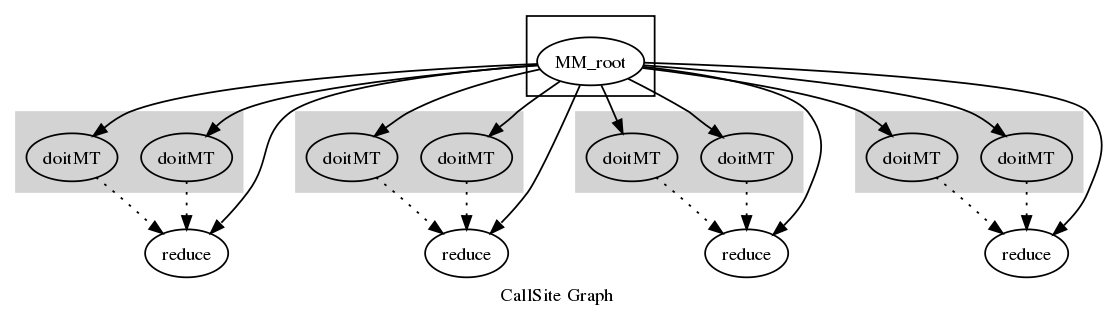
\includegraphics[width=3.3in]{test_matrix}
\caption{MM internal call graph}
\label{fig:mm}
\end{figure}

~\ref{fig:mm} is a cluster of subprocedures generated by libvina after applying \emph{mapreduce} to a matrix multiplication function. Template parameter \_K is 2 in this case because we perform this transform for dual core x86 machine. Libvina \emph{mapreduce} divides a matrix into 4 sub-matrices. The figure except dashed lines is actually a call graph. Shadow lines is multi-threaded environment and two subprocedures are executed in parallel. Dashed lines indicate synchronization logically. 

\emph{mapseq} in \cite{1} can be trivially implemented by passing false to \emph{\_IsMT} parameter. Nested block is possible by recursively defining \emph{TF classes}.

In libvina, programmers only care about developing efficient algorithms. Library takes responsibility for parallelization while keeping the same interface. Porting to another platforms might need to refine template parameters or apply to new template to maintain maximum performance, however, it is unnecessary for programmers to know details of algorithms beneath of the libraries.
\subsection{Pipelining and Streaming}
\subsection{Blocking}
\subsection{Cooperation with other libraries}
We implemented our library in ISO standard C++. Theoretically, any standard-compliance C++ compiler should proceed our classes without trouble. C++0X \cite{17} added a lot of language features to ease template meta-programming. Compilers without C++0X supports need some workarounds to pass compilation. Consider the trend of C++, development libraries such as libvina should be easier in the future. 

We implemented \emph{vina::thread} based on underlying Linux PThread. A simple C++ thread pool is developed to reduce cost of thread creation. SPMD(Single program multiple data) is very important execution model. We utilize OpenCL to execute SPMD programs on GPU. OpenCL framework shipped with Mac OS 10.6 SDK is a library and be totally compatible with our approach. In order to obtain bigger performance on x86, we designed a lightweight thread library(libSPMD) based on Linux clone(2) and semaphore.

\section{Experiment and evaluation}
\subsection{Methodology}
C++0X is partially supported by mainstreaming compilers. Currently, we developed the library for gcc 4.4.0. In order to utilize OpenCL, we modified some codes to satisfied gcc 4.2 for apple. Modifications only increase tediousness of typing and enforce some requirements. They don't affect power of libvina or hurt performance in measurable experiments.

A couple of algorithms are evaluated for libvina.  They are representatives in image processing and scientific computations. 
\begin{itemize}
\item[saxpy] Procedure in BLAS level 1. A scalar multiplies to a single precision vector, which contains 32 million elements.
\item[sgemm] Procedure in BLAS level 3. Two $4096*4096$ dense matrices multiply.
\item[dot\_prod] Two vectors perform dot production.
\item[conv2d] 2-Dimensional convolution operation on image.
\end{itemize}

Three multicore systems are used to conduct experiments. 
\begin{table}[hb]
\caption{Table 1: Experimental machines}
\begin{center}
\begin{tabular}{|l|r|r|l|r|r|}
\hline
name       & ISA         & topology   & frequency  & storage-on-chip & bandwidth      \\
\hline 
harpertown & x86 core 2  & 2-way quad cores & 2.00Ghz & 64K DCache 64K ICache &         \\
           &             &                  &         & 2x 6M shared L2 Cache &         \\
\hline
nehalem    & x86 nehalem & quad cores       & 2.93Ghz & same L1 cache; 256K L2&         \\
           &             &                  &         & 8M shared L3          &         \\
\hline
9400m      & gpu g80     & 16 cores         & 1.10Ghz & 16k local storage     & 3.4Gb/s \\
\hline
\end{tabular} 
\end{center}
\end{table}
On x86 platform, We linked Intel Math kernel library to perform BLAS functions. We implemented convolution 2D and other algorithms on GPU. 

\subsection{Results}
Figures are preparing...
1. speedup\\
2. table: peak performance\\
3. comparison 3 SPMD threads.\\
4. cache misses reduction in blocking\\
5. comparison between gpu and cpu. matrix-multiplications?
\section{Conclusions}
% number - used to balance the columns on the last page
% adjust value as needed - may need to be readjusted if
% the document is modified later
\newpage
\IEEEtriggeratref{11}
% The "triggered" command can be changed if desired:
%\IEEEtriggercmd{\enlargethispage{-5in}}

% references section

% can use a bibliography generated by BibTeX as a .bbl file
% BibTeX documentation can be easily obtained at:
% http://www.ctan.org/tex-archive/biblio/bibtex/contrib/doc/
% The IEEEtran BibTeX style support page is at:
% http://www.michaelshell.org/tex/ieeetran/bibtex/
%\bibliographystyle{IEEEtran}
% argument is your BibTeX string definitions and bibliography database(s)
%\bibliography{IEEEabrv,TCRef.bib}
%
% <OR> manually copy in the resultant .bbl file
% set second argument of \begin to the number of references
% (used to reserve space for the reference number labels box)

\begin{thebibliography}{99}
\setlength{\itemsep}{1mm}
\bibitem{b1} Fatahalian, K., Knight, T., Houston, M., Erez, M., Horn, D.R., Leem, L., Park, J.Y., Ren, M., Aiken, A., Dally, W.J., Hanrahan, P.: Sequoia: Programming The Memory Hierarchy. SC2006
\bibitem{b2} Knight, T. J., Park, J. Y., Ren, M., Houston, M., Erez, M., Fatahalian, K., Aiken, A., Dally, W. J., and Hanrahan, P. Compilation for Explicitly Managed Memory Hierarchies. PPoPP 2007
\bibitem{b3} Aho, A., Sethi, R., Ullman, J.D., Lam, M.: Compilers: Principles, Techniques, and Tools. Addison-Wesley. 
\bibitem{b4} Boehm, H.J.: Threads Cannot Be Implemented As a Library. PLDI '05
\bibitem{b5} Drepper, U., Molnar, I.: The Native POSIX Thread Library for Linux. 2005
\bibitem{b6} Veldhuizen, T. L.: C++ Template are Turing Complete. 
\bibitem{b7} Saha, B., Zhou, X., Chen, H., Gao, Y., Yan, S., Rajagopalan, M., Fang, J., Zhang, P., Ronen, R., Mendelson, A.: Programming Model for Heterogeneous x86 Platform. PLDI '09.
\bibitem{b8} C++ Standard Committee: ISO/IEC 14882:2003(E) Programming Languages — C++, 2003
\bibitem{b9} Alexandrescu, A.: Modern C++ design: generic programming and design patterns applied, 2001
\bibitem{b10} Abrahams, D., Gurtovoy, A.: C++ Template Meta-programming: Concepts, Tools, and Techniques from Boost and Beyond, 2004
\bibitem{b11} Kapasi, U.J., Dally, W.J., Rixner, S., Owens, J.D., Khailany, B.: The Imagine Stream Processor. Proceeding of the 2002 International Conference on Computer Design.
\bibitem{b12} Munshi, A., Khronos OpenCL Working Group, The OpenCL Specification ver.1.0.43, 2009
\bibitem{b13} Goldberg, B.: Functional Programming Language, ACM Computing Surveys, 1996
\bibitem{b14} Seiler, L., Carmean, D., Sprangle, E., Forsyth, T., Abrash, M., Dubey, P., Junkins, S., Lake, A., Sugerman, J., Cavin, R., Espasa, R., Grochowski, E., Juan, T., Hanrahan, P. 2008. Larrabee: A Many–Core x86 Architecture for Visual Computing. ACM Trans. Graph. 27, 3, Article 18 (August 2008), 15 pages. DOI = 10.1145/1360612.1360617 http://doi.acm.org/10.1145/1360612.1360617. 
\bibitem{b15} El-Ghazawi, T., Cantonnet, F., Yao, Y, Rajamony, R.: Developing an Optimized UPC Compiler for Future Architecture
\bibitem{b16} Gurtovoy, A., Abrahams, D.: The BOOST C++ Meta-programming Library
\bibitem{b17} C++ Standard Committee: ISO/IEC DTR 19768 Doc No. 2857, 2009
\end{thebibliography}




% that's all folks
\end{document}


